\documentclass[12pt, a4paper]{article}
    
\usepackage{homework}
\usepackage{amsmath}				% For Math
\usepackage{fancyhdr}				% For fancy header/footer
\usepackage{graphicx}				% For including figure/image
\usepackage{cancel}					% To use the slash to cancel out stuff in work
\usepackage{multirow}

%%%%%%%%%%%%%%%%%%%%%%
% Set up fancy header/footer
\pagestyle{fancy}
\setlength{\headheight}{42pt}
\fancyhead[LO,L]{Name: Yu Ching Hei\\SID: 1155193237\\email: chyu2@cse.cuhk.edu.hk}
\fancyhead[CO,C]{}
\fancyhead[RO,R]{CENG3420 Computer Organization and Design\\Homework 2\\Date: \today}
\fancyfoot[LO,L]{}
\fancyfoot[CO,C]{}
\fancyfoot[RO,R]{Page \thepage}
\renewcommand{\headrulewidth}{0.4pt}
\renewcommand{\footrulewidth}{0.4pt}
%%%%%%%%%%%%%%%%%%%%%%

\begin{document}
\noindent What is your last digit of your SID (0 is regarded as 10)? This value is defined as
NUM\_1 in the whole question paper. (Since my last digit is 7, NUM\_1 is 7)\\

\begin{q}{15}
Consider the following RISC-V instructions. Please note that we treat 
NUM\_1\%2 and NUM\_1\%2+1 as decimal values.
\begin{code}
    li a1, 1    #li a1, NUM_1%2
    li a2, 2    #li a2, NUM_1%2+1
    li a3, 6
    LOOP:
    slti t0, a3, 1
    bne t0, zero, DONE
    add a4, a1, a2
    addi a1, a2, 0
    addi a2, a4, 0
    addi a3, a3, -1
    jal x0, LOOP
    DONE:
    # end of the program
\end{code}
\begin{enumerate}
    \item How many times is the branch instruction executed? (7\%)
    \item What are the final values of a1 and a2. (8\%)
\end{enumerate}
\end{q}

\begin{ans}
    \begin{enumerate}
        \item 7 times, the first 6 times didn't fulfill the check, and the 7$^{\texttt{th}}$ time got the check fulfilled
        \item a1 = 21, a2 = 34 
    \end{enumerate}
\end{ans}
\pagebreak
\begin{q}{20}
Read through the multiplication / devision algorithm: 
\begin{center}
    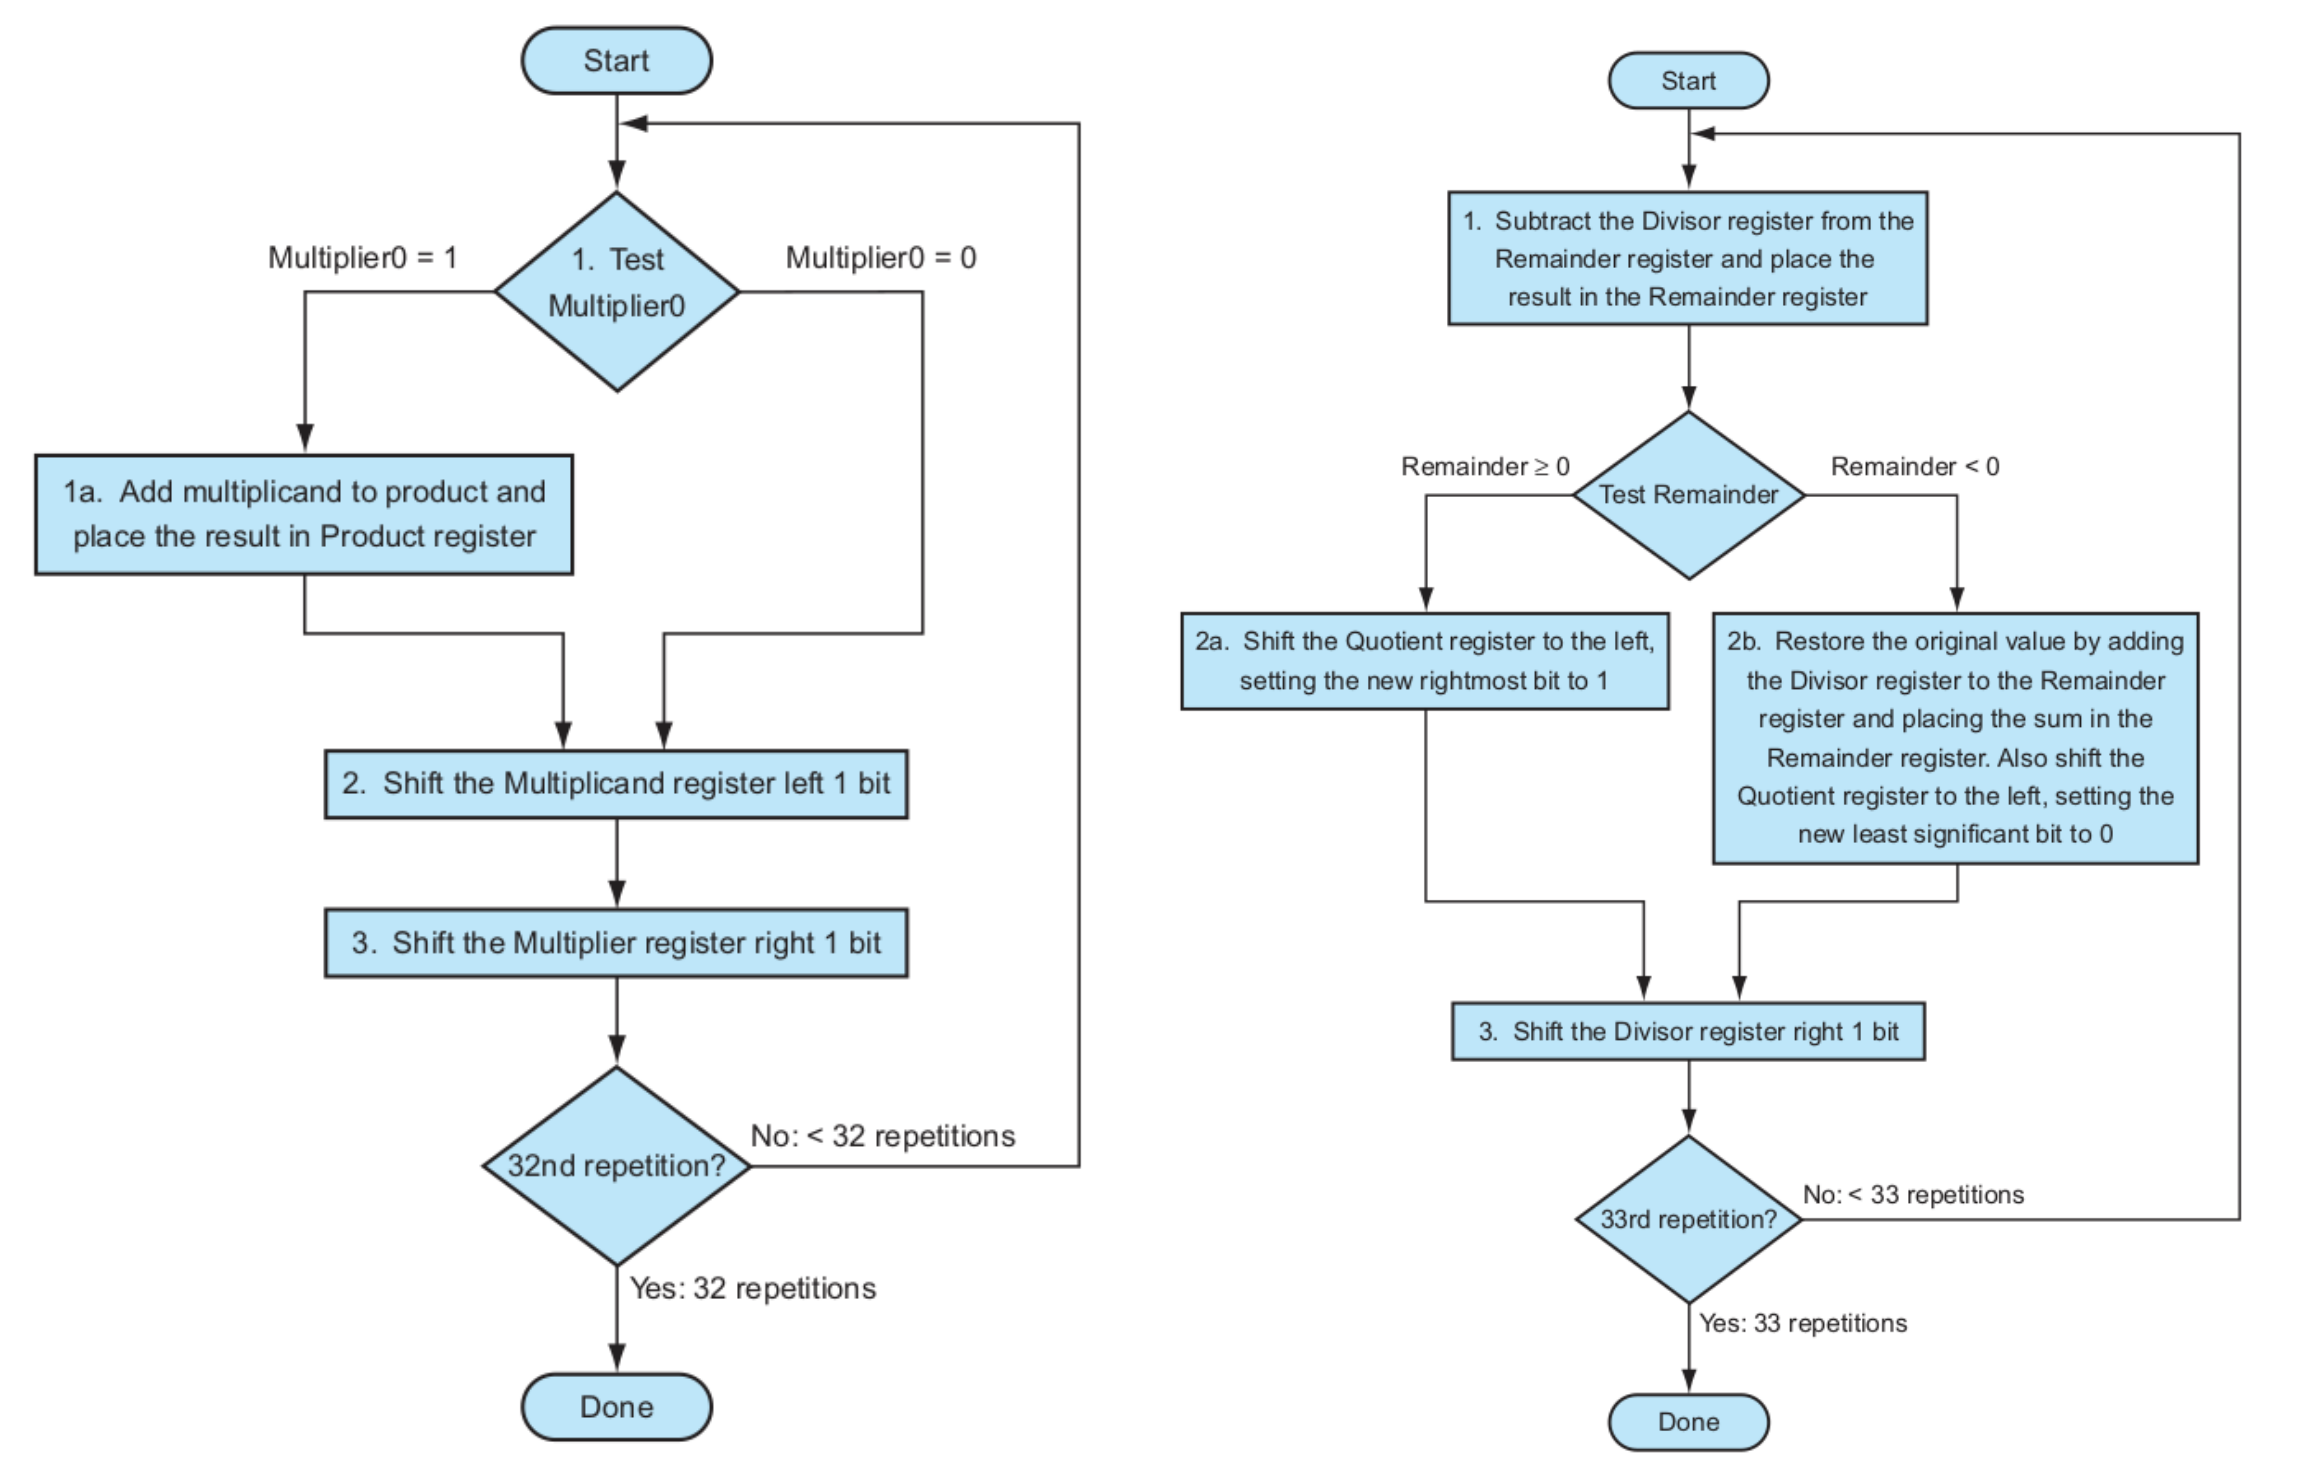
\includegraphics[scale=0.36]{q2.png}
    Left: multiplication algorithm, Right: division algorithm
\end{center}
Write down the step by step procedure to calculate 5×2 or 0101×0010. Use Multiplier0
to indicate the least significant bit of the multiplier. List the initial values and the values
in 1st to 4th iterations of Multiplier, Multiplier0, Multiplicand and Product. In each
iteration, list the values after 1, 2 and 3 steps in Figure 1 left separately. (Represent
Multiplier as 4bits, Multiplier0 as 1bit, Multiplicand as 8bits, Product as 8bits.)
\end{q}
\begin{ans}
    \begin{center}
        \begin{tabular}{|c|c|c|c|c|c|}
            \hline
            Iteration & Step & Multiplier & Multiplier0 & Mcand & Product\\
            \hline
            0 & Initial value & 010\underline{1} & 1 & 0000 0010 & 0000 0000\\
            \hline
            \multirow{3}{*}{1} & \multicolumn{1}{|c}{1$\Rightarrow$Prod=Prod+Mcand} & \multicolumn{1}{|c}{0101} & \multicolumn{1}{|c}{1} & \multicolumn{1}{|c}{0000 0010} & \multicolumn{1}{|c|}{0000 0010} \\\cline{2-6}
                                & \multicolumn{1}{|c}{Shift left Multiplicand} & \multicolumn{1}{|c}{0101} & \multicolumn{1}{|c}{1} & \multicolumn{1}{|c}{0000 0100} & \multicolumn{1}{|c|}{0000 0010} \\\cline{2-6}
                                & \multicolumn{1}{|c}{Shift right Multiplier} & \multicolumn{1}{|c}{001\underline{0}} & \multicolumn{1}{|c}{0} & \multicolumn{1}{|c}{0000 0100} & \multicolumn{1}{|c|}{0000 0010} \\\hline

            \multirow{2}{*}{2} 
                                & \multicolumn{1}{|c}{Shift left Multiplicand} & \multicolumn{1}{|c}{0010} & \multicolumn{1}{|c}{0} & \multicolumn{1}{|c}{0000 1000} & \multicolumn{1}{|c|}{0000 0010} \\\cline{2-6}
                                & \multicolumn{1}{|c}{Shift right Multiplier} & \multicolumn{1}{|c}{000\underline{1}} & \multicolumn{1}{|c}{1} & \multicolumn{1}{|c}{0000 1000} & \multicolumn{1}{|c|}{0000 0010} \\\hline

            \multirow{3}{*}{3} & \multicolumn{1}{|c}{1$\Rightarrow$Prod=Prod+Mcand} & \multicolumn{1}{|c}{0001} & \multicolumn{1}{|c}{1} & \multicolumn{1}{|c}{0000 1000} & \multicolumn{1}{|c|}{0000 1010} \\\cline{2-6}
                                & \multicolumn{1}{|c}{Shift left Multiplicand} & \multicolumn{1}{|c}{0001} & \multicolumn{1}{|c}{1} & \multicolumn{1}{|c}{0001 0000} & \multicolumn{1}{|c|}{0000 1010} \\\cline{2-6}
                                & \multicolumn{1}{|c}{Shift right Multiplier} & \multicolumn{1}{|c}{000\underline{0}} & \multicolumn{1}{|c}{0} & \multicolumn{1}{|c}{0001 0000} & \multicolumn{1}{|c|}{0000 1010} \\\hline

            \multirow{2}{*}{4}
                                & \multicolumn{1}{|c}{Shift left Multiplicand} & \multicolumn{1}{|c}{000\underline{0}} & \multicolumn{1}{|c}{0} & \multicolumn{1}{|c}{0010 0000} & \multicolumn{1}{|c|}{0000 1010} \\\cline{2-6}
                                & \multicolumn{1}{|c}{Shift right Multiplier} & \multicolumn{1}{|c}{000\underline{0}} & \multicolumn{1}{|c}{0} & \multicolumn{1}{|c}{0010 0000} & \multicolumn{1}{|c|}{0000 1010} \\\hline
        \end{tabular}
    \end{center}
\end{ans}
\pagebreak

\begin{q}{20}
    IEEE 754 Floating-Point Standard
    \begin{enumerate}
        \item What decimal number does this single precision float $\mathtt{C13C0000_{16}}$ represent? (Show your work.) (10 \%)
        \item What is -1.5$_{10}$ in IEEE single precision binary floating point format? (Show your work.) (10\%)
    \end{enumerate}
\end{q}
\begin{ans}
    \begin{enumerate}
        \item \begin{enumerate}
                \item by breaking the hexadecimal number into binary, we get $$\mathtt{C13C0000_{16}}=\mathtt{1100 0001 0011 1100 0000 0000 0000 0000_2}$$
                \item the first bit indicate the sign, in this case it is a negative number
                \item the next 8 bits are used to express the exponent of 2 offset by -127, so the exponent in this case is $\mathtt{10000010_2 - 127_{10} = 130_{10} - 127_{10} = 3_{10}}$ 
                \item the following 23 bits($\mathtt{011 1100 0000 0000 0000 0000_2}$) are the mantissa which is a decimal number with a leading 1. i.e. $\mathtt{1.01111_2}$, it is then shift right by times of the exponent and therefore $\mathtt{-1011.11_2}$
                \item $\mathtt{1011_2 = 11_{10}}$ \& $\mathtt{0.11_2 = 0.5 + 0.25 = 0.75_{10}}$ 
            \end{enumerate}
            \begin{center}
                $\therefore-11.75_{10}$
            \end{center}
        \item \begin{enumerate}
                \item Since it is negative, the first bit is 1
                \item Since the part before the decimal point is -1 only, there is no need to shift the bits exponent = 127
                \item then convert the number after the decimal point by multiplying 2 and extract the decimal number, 
                        $$0.5 \times 2 = \underline{1}.0 \Rightarrow 1$$
                    so we have mantissa 100 0000 0000 0000 0000 0000
                \item so the single precision floating point number is
                    \begin{center}
                        1 01111111 10000000000000000000000$_2$ = BFC00000$_{16}$
                    \end{center}
            \end{enumerate}
    \end{enumerate}
\end{ans}
\pagebreak
\begin{q}{10}
Consider the following instruction:\\
Instruction: \texttt{xor rd, rs1, rs2}\\
Interpretation: \texttt{Reg[rd] = Reg[rs1] XOR Reg[rs2]}
\begin{enumerate}
    \item What are the values of control signals generated by the control in figure 2 for this
    instruction?
    \item Which resource (block) produces no output for this instruction?
\end{enumerate}
\begin{center}
    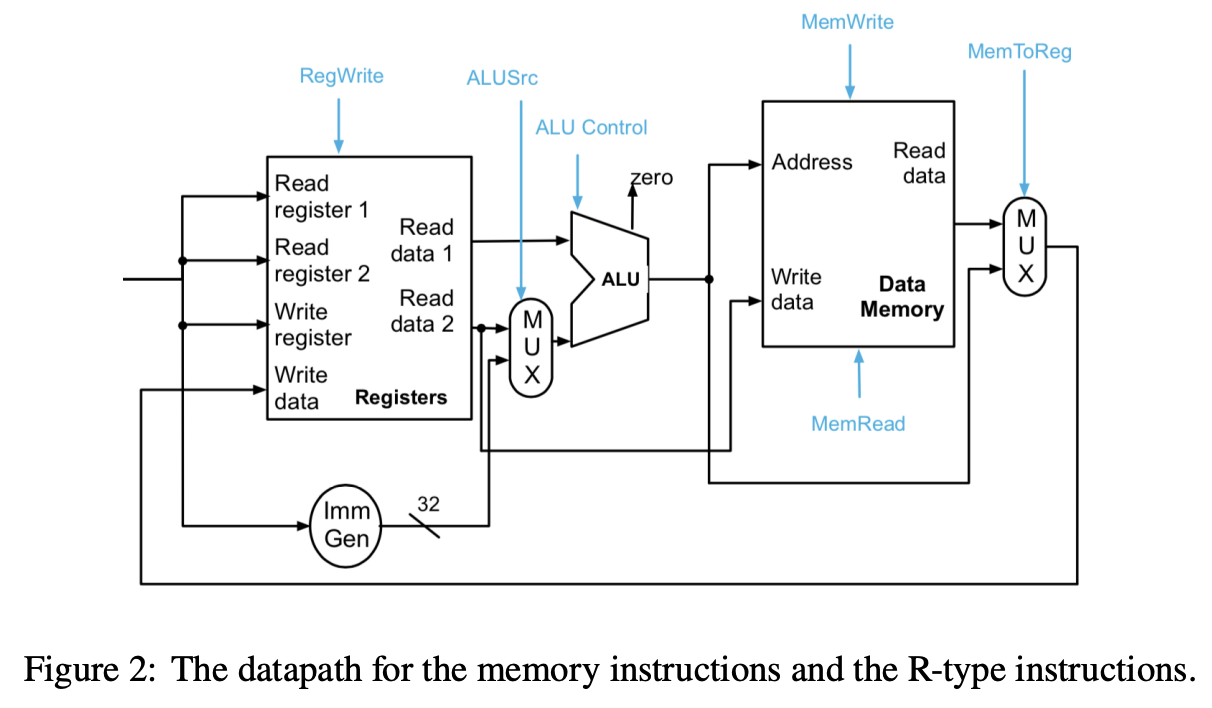
\includegraphics[scale=0.65]{q3.png}
\end{center}
\end{q}
\begin{ans}
    \begin{enumerate}
        \item RegWrite = true, ALUSrc = 0, ALU Control = "xor", MemWrite = false, \\MemRead = false, MemToReg = 0 
        \item Data Memory
    \end{enumerate}
\end{ans}
\pagebreak
\begin{q}{15}
The following figures show the format and datapath of an R format instruction.
\centering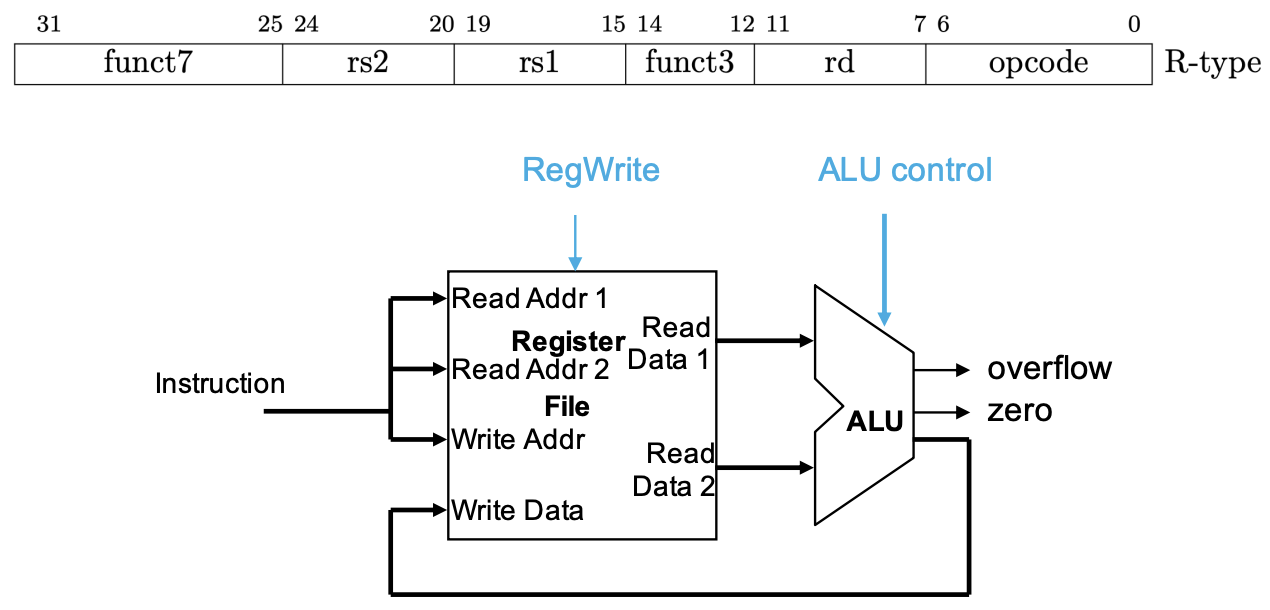
\includegraphics[scale=0.65]{q5.png}
\begin{enumerate}
    \item Assume we have an instruction whose machine code is 0x00c5d533, please write
    down the instruction in assembly language. (10\%)
    \item Which ports in the datapath do we use for addressing rs1, rs2, and rd? (5\%)
\end{enumerate}
\end{q}
\begin{ans}
    \begin{enumerate}
        \item By breaking down the machine code, it is 0000 0000 1100 0101 1101 0101 0011 0011$_2$. 
                \begin{enumerate}
                    \item By bit0-7(0110011), we can know that it is a R-type instruction. 
                    \item By bit7-11(01010), we can know that rd is x10 which is a0.
                    \item By ``funct3'' (bit12-14 = $101_2$ = 0x5), we know that it is a shift right function. 
                    \item By bit15-19(01011) we can know that r1 is x11 which is a1.
                    \item By bit20-24(01100) we can know that r2 is a2. 
                    \item By ``funct7''(bit25-31 = 0000000$_2$ = 0), so we can know that it is a shift right logical function. 
                \end{enumerate}
                Therefore the code instruction in assembly is:
                \begin{verbatim}
                    srl a0, a1, a2
                \end{verbatim}
        \item 
        \begin{itemize}
            \item Read Addr 1: rs1
            \item Read Addr 2: rs2
            \item Write Addr: rd
        \end{itemize}
    \end{enumerate}
\end{ans}
\pagebreak
\begin{q}{20}
In this exercise, we examine how pipelining affects the clock cycle time of the 
processor. Problems in this exercise assume that individual stages of the datapath 
have the following latencies:
\begin{center}
    \begin{tabular}{|c|c|c|c|c|}
        \hline
        \bf{IF} & \bf{ID} & \bf{EX} & \bf{MEM} & \bf{WB}\\
        \hline
        300ps & 500ps & 200ps & 350ps & 250ps\\
        \hline
    \end{tabular}
\end{center}
\begin{enumerate}
    \item What is the clock cycle time in a pipelined and non-pipelined (single-cycle) processor?
    \item What is the total latency of an lw instruction in a pipelined and non-pipelined
    (single-cycle) processor?
    \item If we can split one stage of the pipelined datapath into two new stages, each with
    half the latency of the original stage, which stage would you split and what is the
    new clock cycle time of the processor?
\end{enumerate}
\end{q}
\begin{ans}
    \begin{enumerate}
        \item Clock cycle time: 
            \begin{itemize}
                \item pipelined: max(300, 500, 200, 350, 250) = 500ps
                \item non-pipelined: $300+500+200+350+250=1600$ps
            \end{itemize}
        \item Total latency: 
            \begin{itemize}
                \item pipelined: $500 \times 5 = 2500$ps
                \item non-pipelined: Single clock cycle time = 1600ps
            \end{itemize}
        \item I would split the stage ``ID'' as it has the longest latency which ``EX'' and ``WB''only occupies less than or equal to half of its latency. \\
        New clock cycle time = 350ps
    \end{enumerate}
\end{ans}
\end{document}
